\chapter{Introduction}
This is the final report for the senior thesis design course offered by the \gls{ceen} department of the University of Nebraska-Lincoln.
The team chose to design and create a \gls{cnc} interface that has been nicknamed the \gls{ceenc}.

\section{Problem Statement}
The \gls{ceenc} is a web-enabled \gls{cnc} interface designed with students and hobbyists in mind.
Most modern \gls{cnc} interfaces and drivers are large and expensive, making it difficult for students, hobbyists, and smaller companies to own a \gls{cnc}.
The \gls{ceenc} is an affordable and compact device, enabling users to cut down on project development time and cost.
The device can also be configured for multiple setups, including linear \gls{cnc}s, delta robots, or a \gls{3d} printer.
The web interface also improves upon connectivity, allowing the device to be used from anywhere on the network.

\section{Objectives}
The purpose of the \gls{ceenc} project is to create a \gls{cnc} interface, capable of receiving standardized G-code through	 \gls{tcpip}, processing the G-code, and driving motors and general purpose outputs according to the G-code.
G-code is a standard \gls{cnc} programming language, but is more complicated than accepting individual commands to move the motors.
Figure ~\ref{fig:o-tree} shows the objective tree for the \gls{ceenc}, showing the importance of safety and \gls{cnc} functionality.
The numbers referencing \gls{pssc}s are described in ~\ref{sec:psscs}.

\begin{figure}[h]
	\centering
	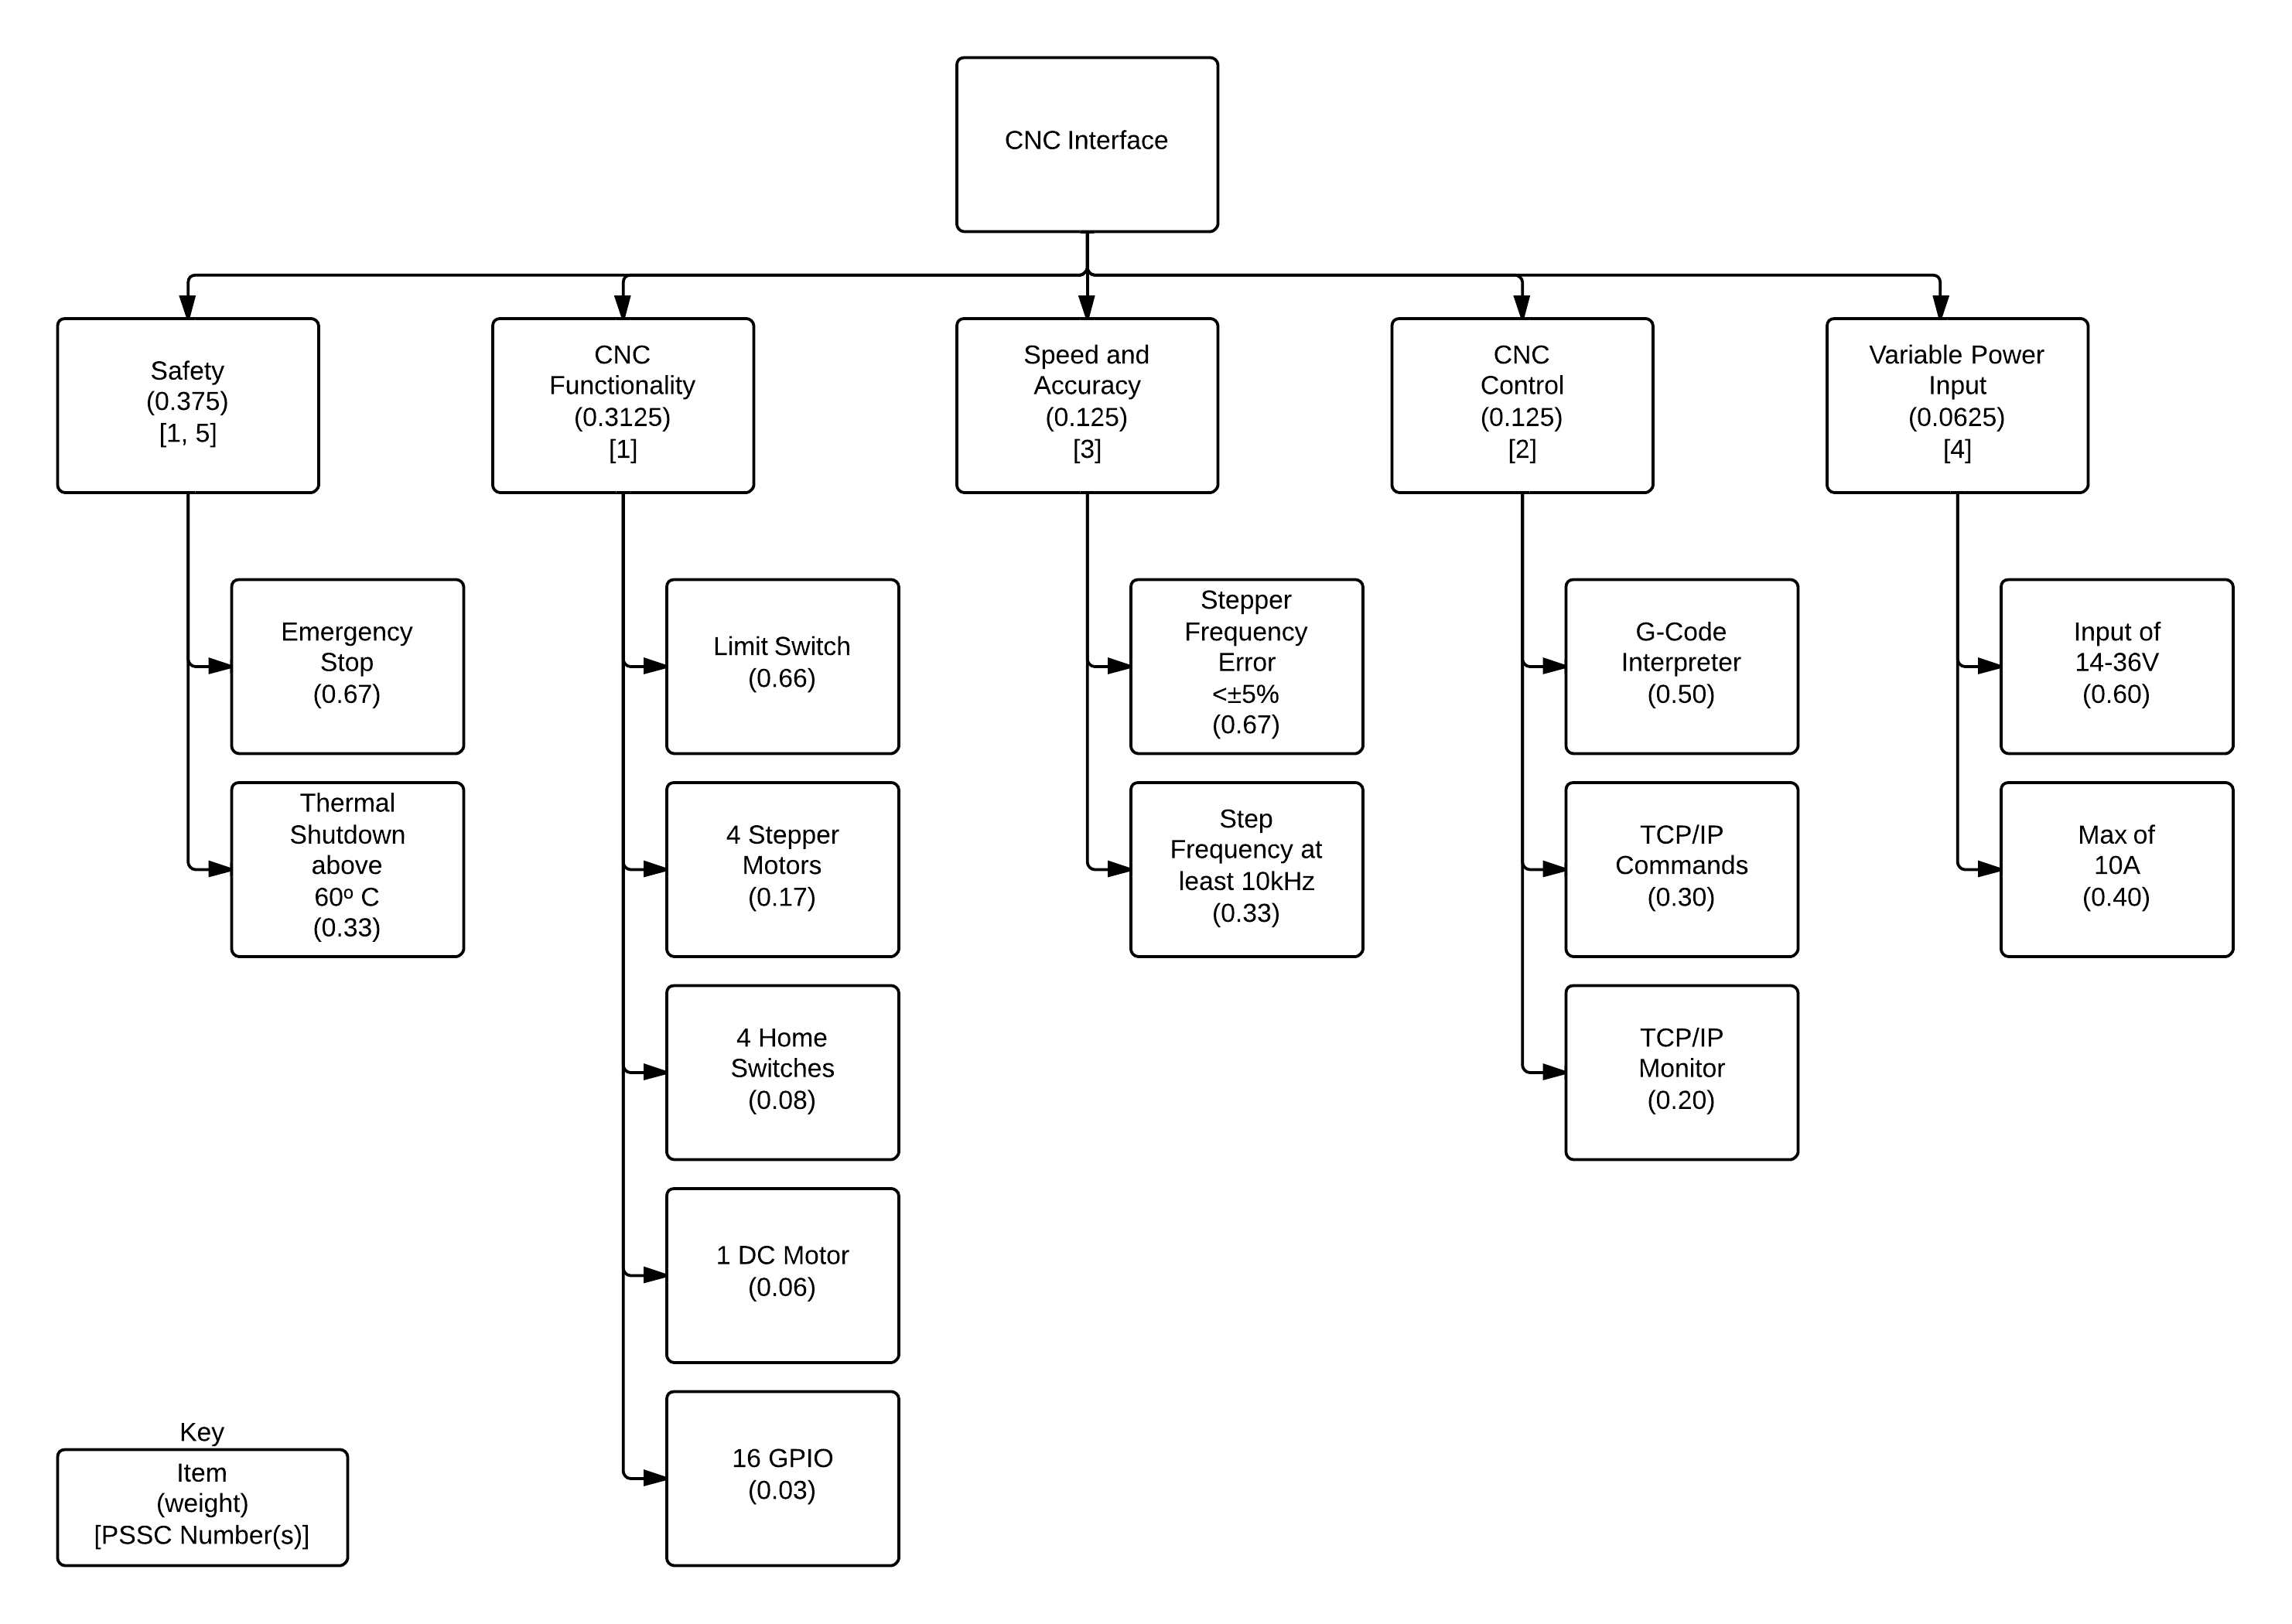
\includegraphics[width=1\textwidth]{objective-tree.png}
	\caption{Objective Tree}
	\label{fig:o-tree}
\end{figure}

\section{Report Format}
This report discusses the need for the product, the solution design process, the implemented solution and how it works, and how the solutions may affect the world.
Final recommendations are given for future enhancements for the project to move forward and continue improving.
